\documentclass[a4paper]{article}

%% Language and font encodings
\usepackage[english]{babel}
\usepackage[utf8x]{inputenc}
\usepackage[T1]{fontenc}

%% Sets page size and margins
\usepackage[a4paper,top=3cm,bottom=2cm,left=3cm,right=3cm,marginparwidth=1.75cm]{geometry}

%% Useful packages
\usepackage{amsmath}
\usepackage{graphicx}
\usepackage[colorinlistoftodos]{todonotes}
\usepackage[colorlinks=true, allcolors=blue]{hyperref}

\title{4th Paper: Optimal Grid Design in Operating Models: Work smarter, not harder}
\author{Iago Mosqueira, Rishi Sharma, Laurie Kell, Toshihide  Kitakado}

\begin{document}
\maketitle

\begin{abstract}
MSE's often use assessment models with complex structural uncertainty designs examining multiway interactions. The paper examines different approaches to evaluate multi-way interactions and optimize grid design to capture the uncertainty in the system being modeled. The objective is not to make a perfect assessment model, but rather to capture the true dynamics of teh system that encapsulates the underlying uncertainty so a reference set along with a robustness set of models could be examined to optimize a control rule that coud be empirical or model based in nature.

\end{abstract}

\section{Introduction}

MSE’s often use complicated grid based platforms to test alternative states of nature (e.g. CCSBT, Hillary et al. 2016 ). This was the case in initial development for Albacore in the Indian Ocean (Mosqueira and Sharma 2014 IOTC 2014-WPM 05) based on the Synthesis Assessment (Hoyle et. al. 2014). In that case 720 models were examined as the basis of the operating model. However, in the case of the Atlantic (Kell et. al. 2016), a much finer operating model structure was used (10 models) conditioned on the MultiFan Assessment (Anon 2012).  Thus, a whole range of approaches is available in the literature (Punt et. al. 2014) and we would examine if a full grid approach is relevant, or something simpler could work. 
The objective of this work is to first examine the grid structure using GLM based methods to determine which variables effect the derived parameters like B0 and current stock size. Once the main and interaction effects that are important are figured a refined grid could be examined.
In addition, the variance covariance matrix produced by the assessment and test whether we need a complex model structure for the MSE (CCSBT and IOTC) or do simpler structures perform just as well (ICCAT). We would use the Synthesis model and platform to examine this (with the Indian Ocean Albacore Assessment). Tools already developed (Mosqueira and Sharma 2014) could be further developed to examine across SS model platforms and to make it more generic for application in other assessments in the Atlantic. 
The objective here is to examine whether main effects used in the grid are sufficient for robustness testing of the MP, and provide adequate contrast in the states of nature or do we need to apply all possible interactions in the grid as well, and can the variance co-variance matrix inform us of the scenarios that could be used.


\section{Some examples to get started}

\subsection{How to include Figures}

First you have to upload the image file from your computer using the upload link the project menu. Then use the includegraphics command to include it in your document. Use the figure environment and the caption command to add a number and a caption to your figure. See the code for Figure \ref{fig:frog} in this section for an example.

\begin{figure}
\centering
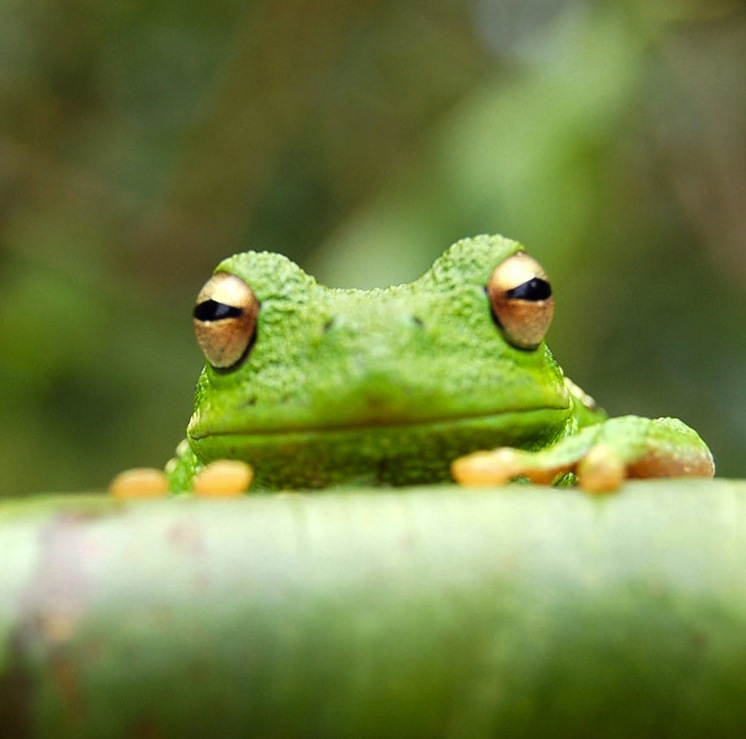
\includegraphics[width=0.3\textwidth]{frog.jpg}
\caption{\label{fig:frog}This frog was uploaded via the project menu.}
\end{figure}

\subsection{How to add Comments}

Comments can be added to your project by clicking on the comment icon in the toolbar above. % * <john.hammersley@gmail.com> 2016-07-03T09:54:16.211Z:
%
% Here's an example comment!
%
To reply to a comment, simply click the reply button in the lower right corner of the comment, and you can close them when you're done.

Comments can also be added to the margins of the compiled PDF using the todo command\todo{Here's a comment in the margin!}, as shown in the example on the right. You can also add inline comments:

\todo[inline, color=green!40]{This is an inline comment.}

\subsection{How to add Tables}

Use the table and tabular commands for basic tables --- see Table~\ref{tab:widgets}, for example. 

\begin{table}
\centering
\begin{tabular}{l|r}
Item & Quantity \\\hline
Widgets & 42 \\
Gadgets & 13
\end{tabular}
\caption{\label{tab:widgets}An example table.}
\end{table}

\subsection{How to write Mathematics}

\LaTeX{} is great at typesetting mathematics. Let $X_1, X_2, \ldots, X_n$ be a sequence of independent and identically distributed random variables with $\text{E}[X_i] = \mu$ and $\text{Var}[X_i] = \sigma^2 < \infty$, and let
\[S_n = \frac{X_1 + X_2 + \cdots + X_n}{n}
      = \frac{1}{n}\sum_{i}^{n} X_i\]
denote their mean. Then as $n$ approaches infinity, the random variables $\sqrt{n}(S_n - \mu)$ converge in distribution to a normal $\mathcal{N}(0, \sigma^2)$.


\subsection{How to create Sections and Subsections}

Use section and subsections to organize your document. Simply use the section and subsection buttons in the toolbar to create them, and we'll handle all the formatting and numbering automatically.

\subsection{How to add Lists}

You can make lists with automatic numbering \dots

\begin{enumerate}
\item Like this,
\item and like this.
\end{enumerate}
\dots or bullet points \dots
\begin{itemize}
\item Like this,
\item and like this.
\end{itemize}

\subsection{How to add Citations and a References List}

You can upload a \verb|.bib| file containing your BibTeX entries, created with JabRef; or import your \href{https://www.overleaf.com/blog/184}{Mendeley}, CiteULike or Zotero library as a \verb|.bib| file. You can then cite entries from it, like this: \cite{greenwade93}. Just remember to specify a bibliography style, as well as the filename of the \verb|.bib|.

You can find a \href{https://www.overleaf.com/help/97-how-to-include-a-bibliography-using-bibtex}{video tutorial here} to learn more about BibTeX.

We hope you find Overleaf useful, and please let us know if you have any feedback using the help menu above --- or use the contact form at \url{https://www.overleaf.com/contact}!

\bibliographystyle{alpha}
\bibliography{sample}

\end{document}